\section{\name Prototype Implementation}
\label{sec:prototype}


\begin{figure}[t]
\centering
%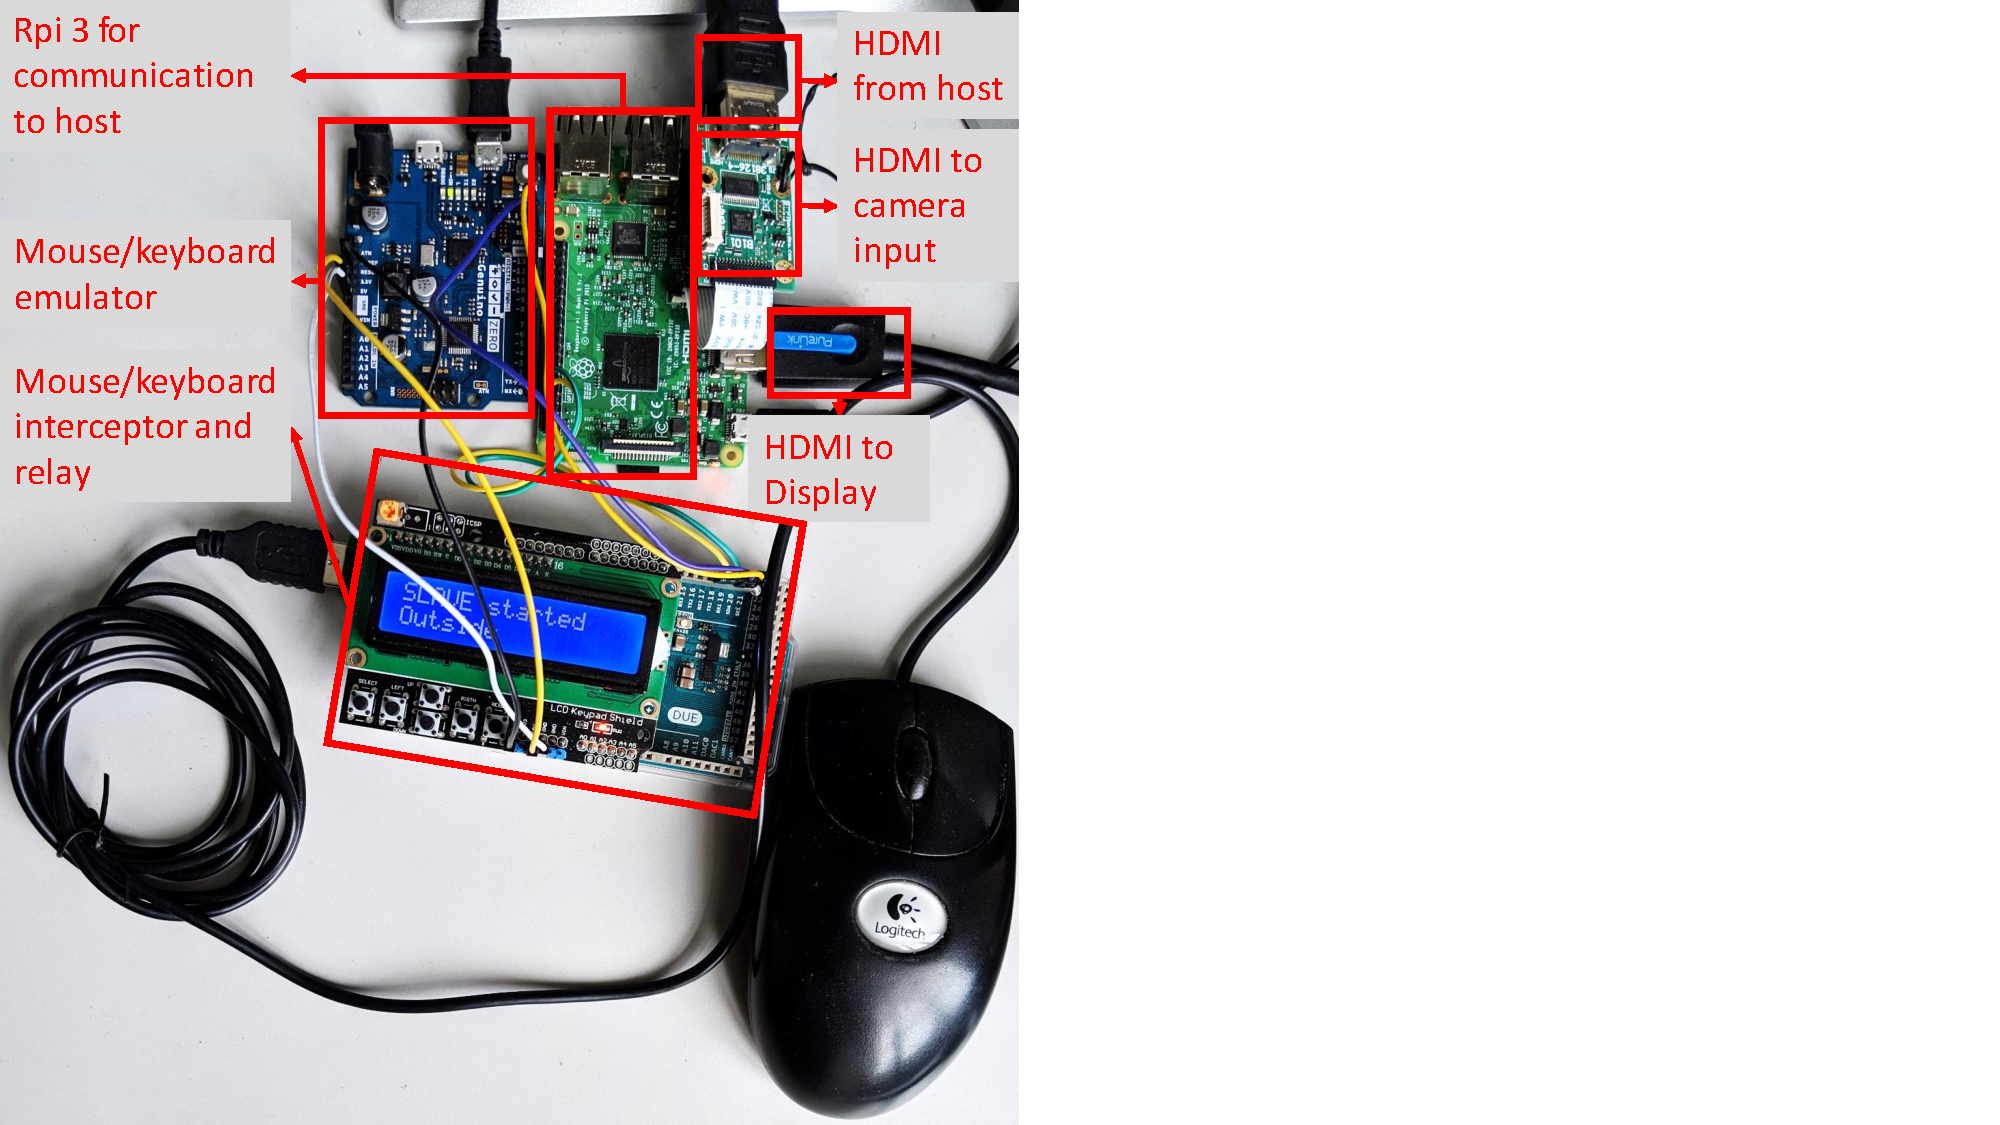
\includegraphics[trim={0 0 15cm 0}, clip, width=\linewidth]{setUp.pdf}
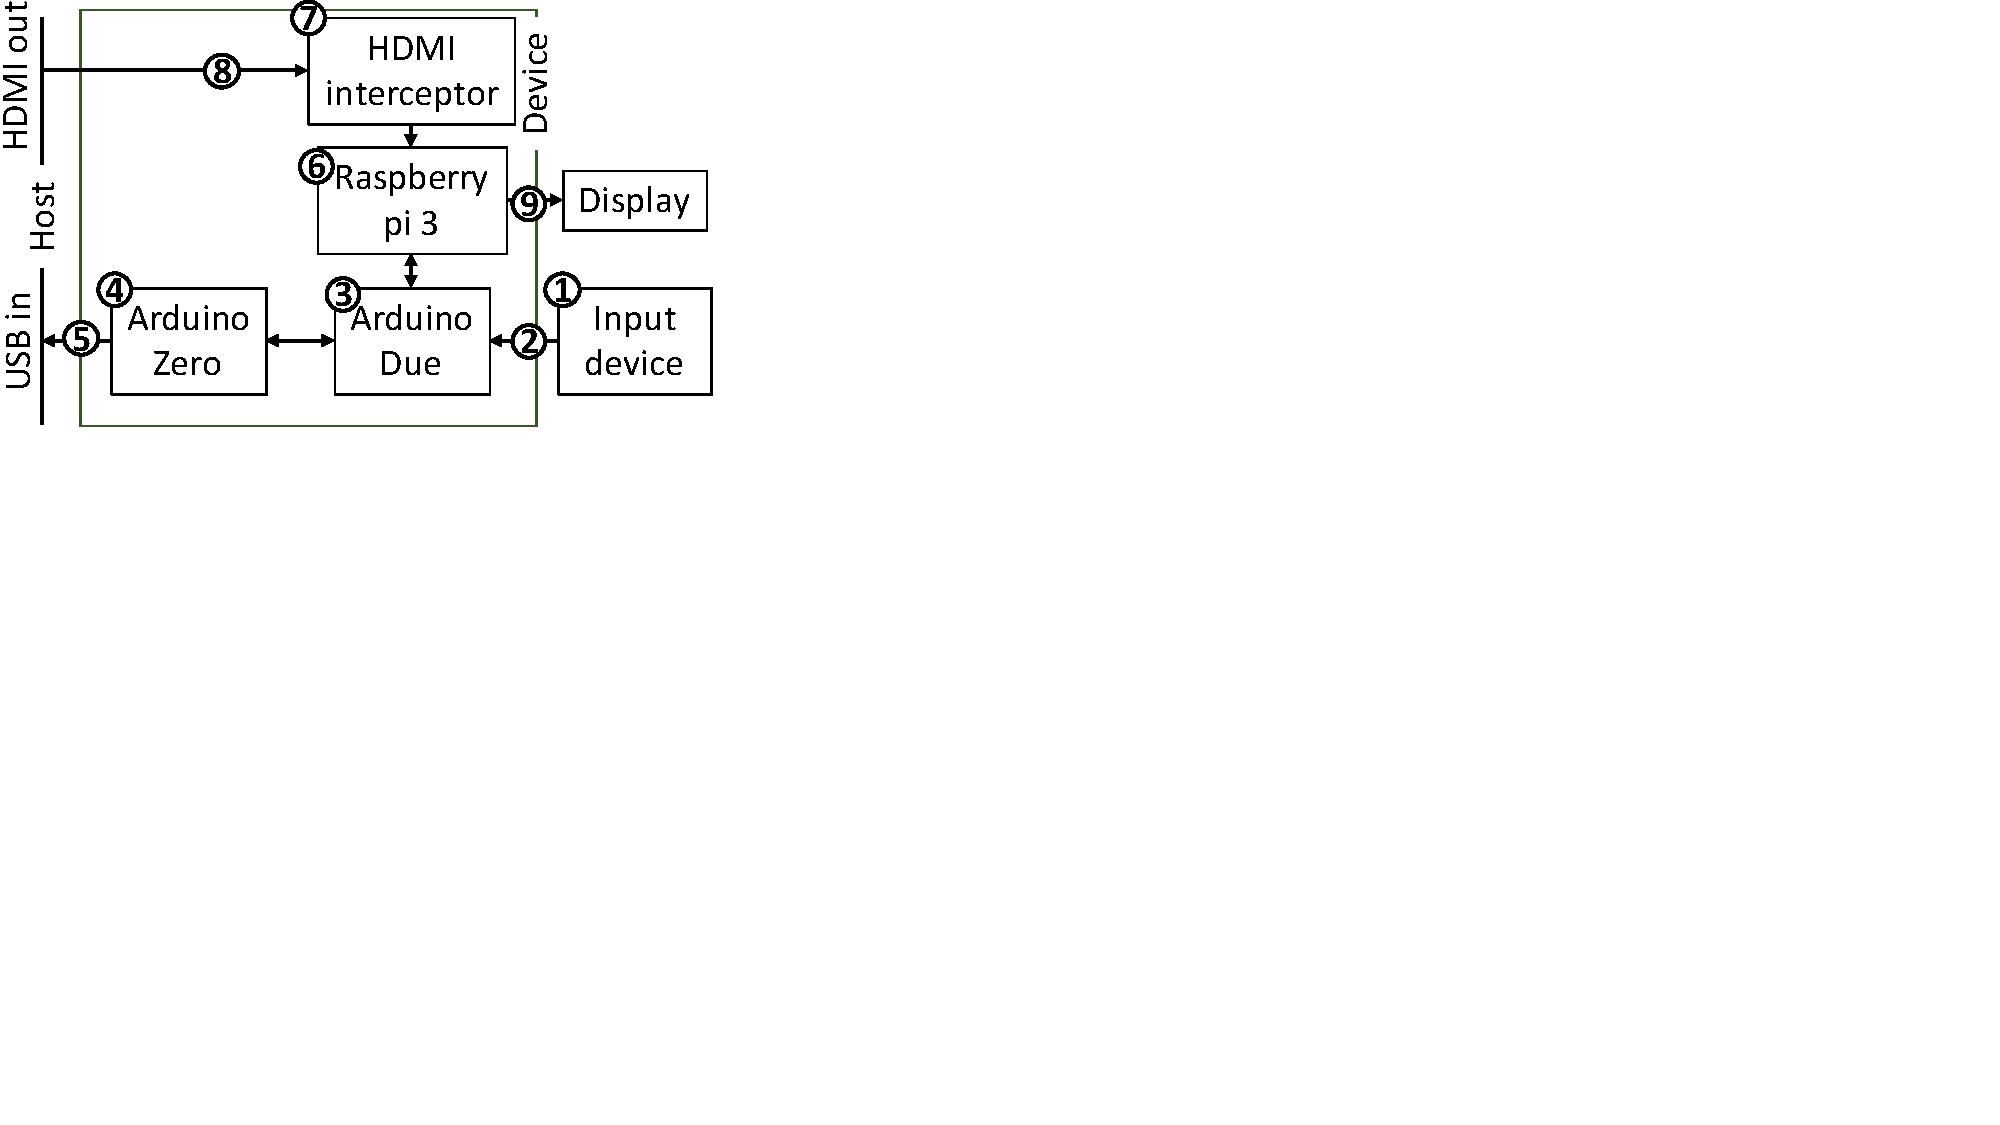
\includegraphics[trim={0 12cm 21.7cm 0}, clip, width=0.7\linewidth]{setUpBlock.pdf}
\caption{\textbf{\name prototype architecture}. }
\label{fig:prototypeArch}
\centering
\end{figure}


\begin{figure}[t]
\centering
%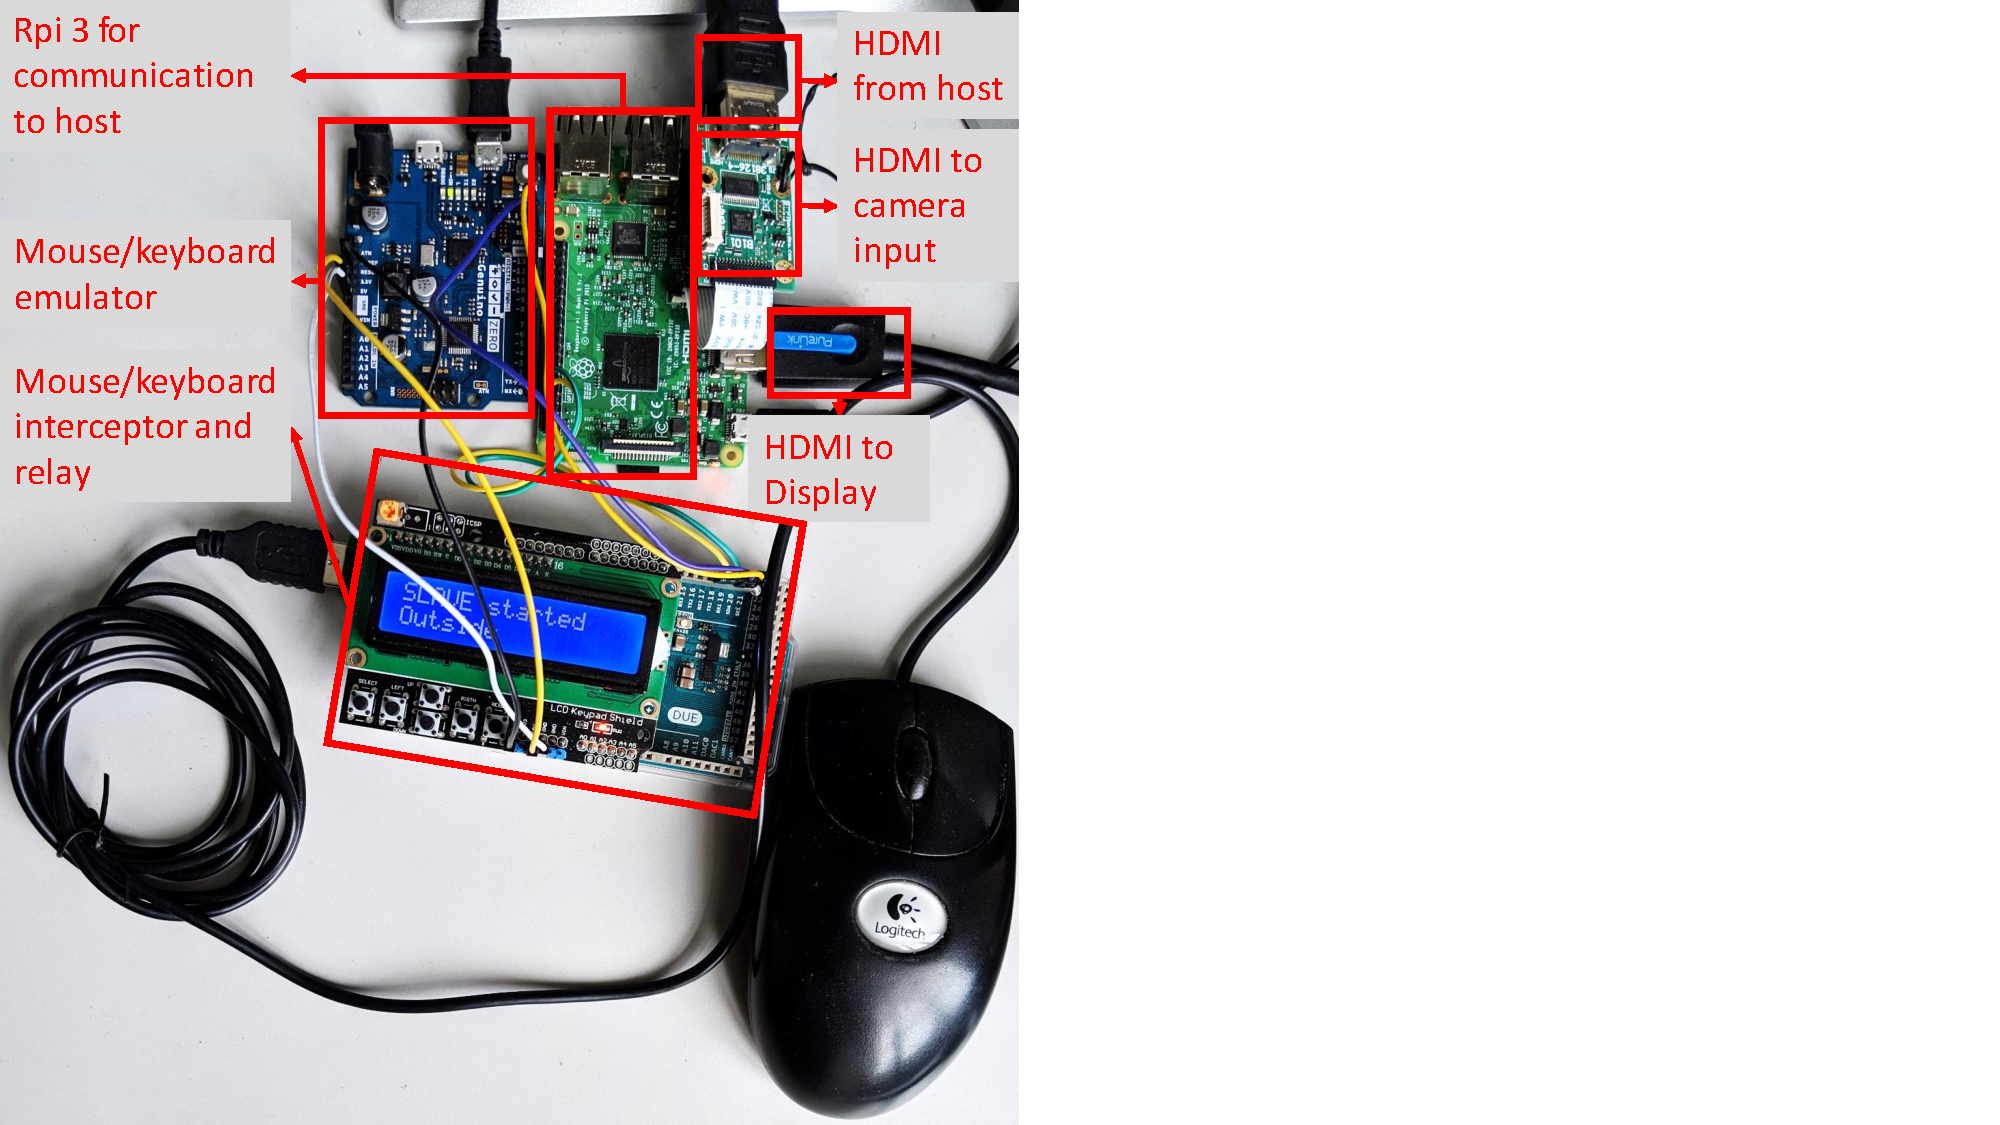
\includegraphics[trim={0 0 15cm 0}, clip, width=\linewidth]{setUp.pdf}
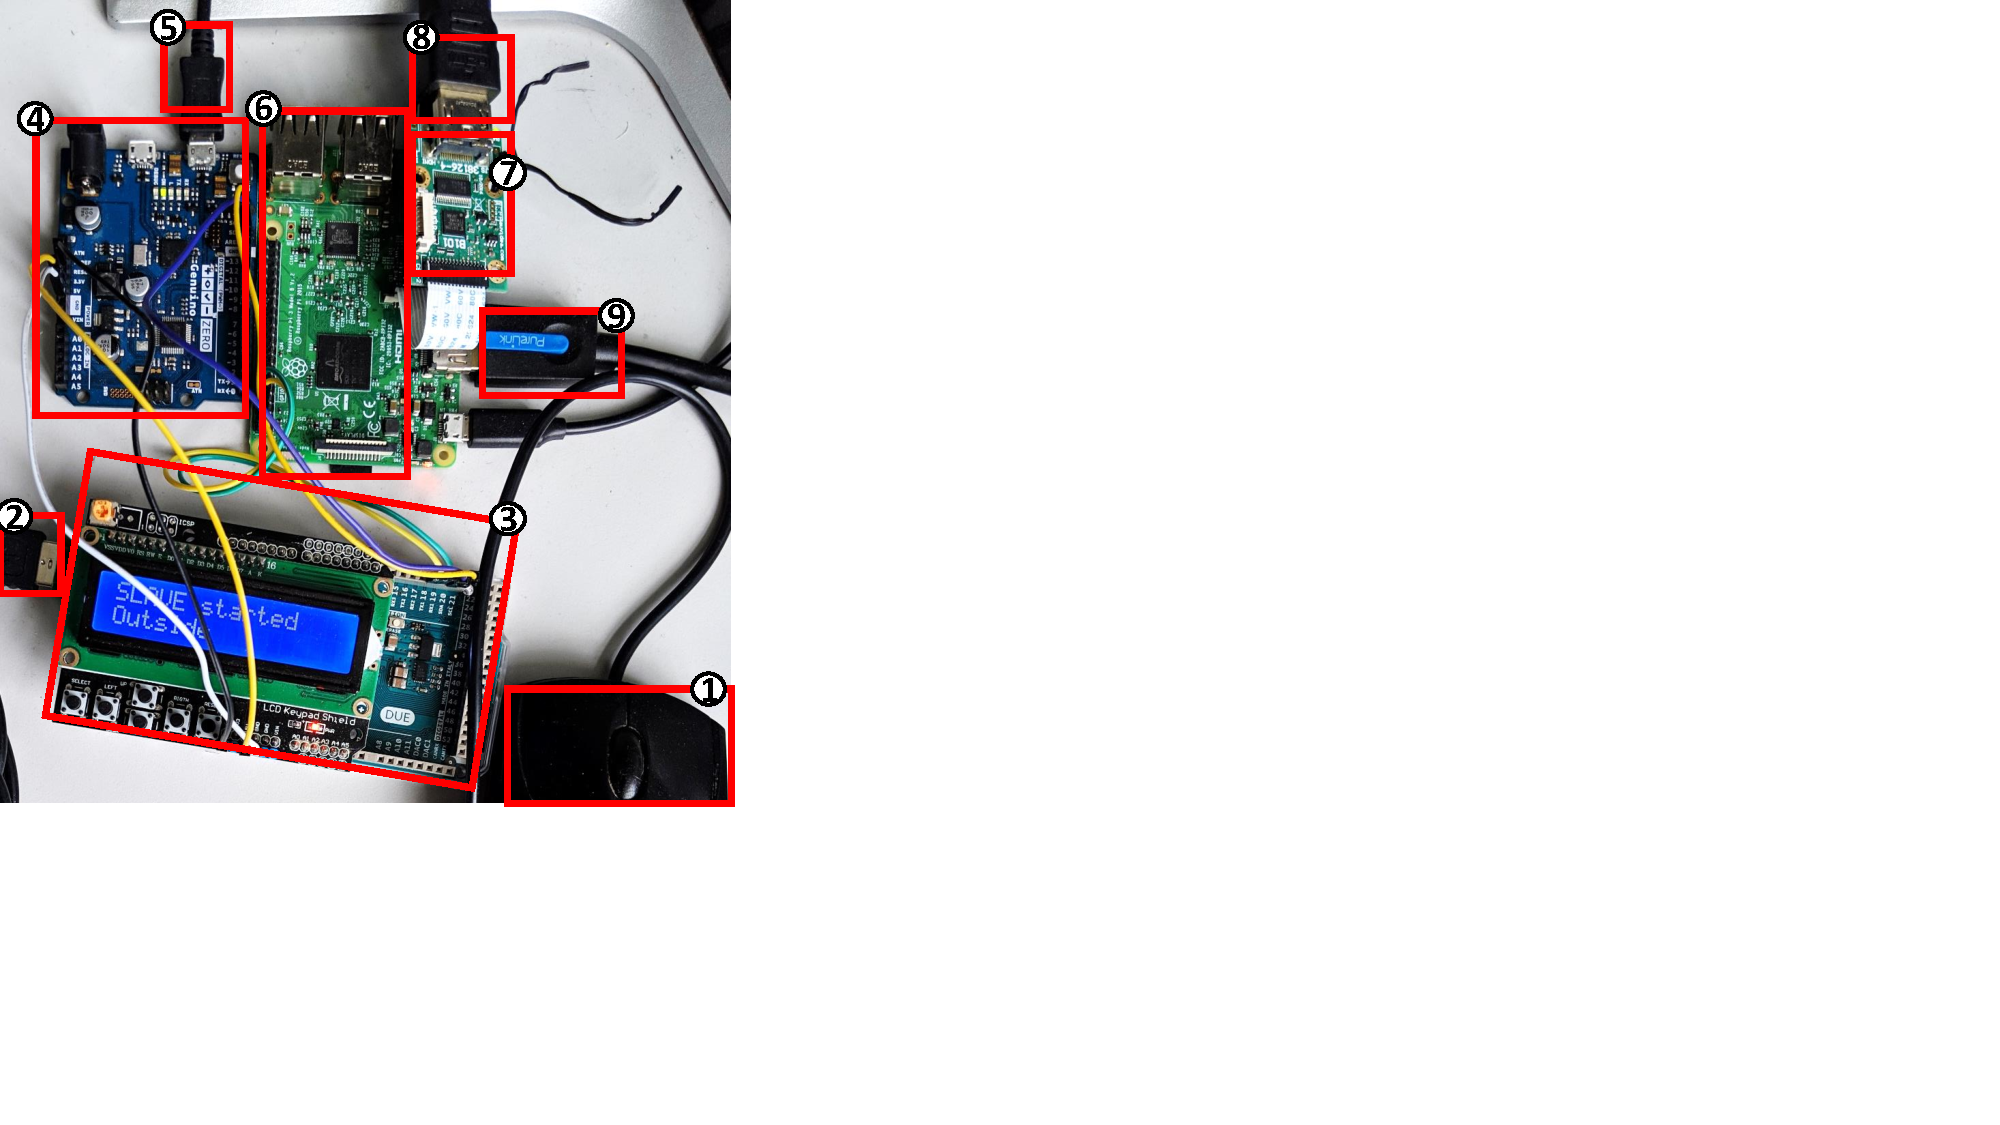
\includegraphics[trim={0 5cm 21.5cm 0}, clip, width=0.75\linewidth]{setUp_1.pdf}
\caption{\textbf{\name prototype}. The figure shows \name prototype that employs Arduino Due and Zero microcontroller board and a Raspberry Pi 3 SBC. The highlighted numbers correspond to the labels in Figure~\ref{fig:prototypeArch}.}
\label{fig:prototype}
\centering
\end{figure}

In this section, we describe our prototype implementation of \name as an auxiliary device. Figure~\ref{fig:prototype} depicts the \name prototype that has the following components

\begin{enumerate}
  \item \textbf{IO interceptor.} The IO interceptor is composed of a  
  \item \textbf{HDMI interceptor.} 
\end{enumerate}